\documentclass[9pt,twocolumn,twoside,lineno]{pnas-new}
% Use the lineno option to display guide line numbers if required.

\templatetype{pnasresearcharticle} % Choose template 
% {pnasresearcharticle} = Template for a two-column research article
% {pnasmathematics} %= Template for a one-column mathematics article
% {pnasinvited} %= Template for a PNAS invited submission

\usepackage{amsmath}
\usepackage{tikz-dependency}
\DeclareMathOperator*{\argmax}{arg\,max}
\DeclareMathOperator*{\argmin}{arg\,min}
\DeclareMathOperator{\E}{\mathop{\mathbb{E}}}

\usepackage{amssymb}% http://ctan.org/pkg/amssymb
\usepackage{pifont}% http://ctan.org/pkg/pifont
\newcommand{\cmark}{\ding{51}}%
\newcommand{\xmark}{\ding{55}}%


%https://tex.stackexchange.com/questions/219676/how-to-change-spacing-before-and-after-paragraph-command
%\usepackage{xpatch}

%\usepackage{pslatex}
%\usepackage{latexsym}
\usepackage[english]{babel}
\usepackage[utf8]{inputenc}
\usepackage{bm}
\usepackage{graphicx}
\usepackage{tikz}
\usepackage{xcolor}
\usepackage{url}
%\usepackage[colorinlistoftodos]{todonotes}
\usepackage{rotating}
\usepackage{multirow}

\newcommand{\R}[0]{\mathbb{R}}
\newcommand{\Ff}[0]{\mathcal{F}}
\newcommand{\key}[1]{\textbf{#1}}


\newcommand{\soft}[1]{}
\newcommand{\nopreview}[1]{}
\newcommand\comment[1]{{\color{red}#1}}
\newcommand\mhahn[1]{{\color{red}(#1)}}
\newcommand{\rljf}[1]{{\color{blue}[rljf: #1]}}

\newcommand{\thetad}[0]{{\theta_d}}
\newcommand{\thetal}[0]{{\theta_{LM}}}
\newcommand{\thetap}[0]{{\theta_{P}}}


\renewcommand{\baselinestretch}{0.99}
\addtolength{\textfloatsep}{-0.18in}
\setlength{\abovecaptionskip}{5pt plus 1pt minus 0pt} % Chosen fairly arbitrarily
%\setlength{\belowcaptionskip}{-5pt}
%https://tex.stackexchange.com/questions/23313/how-can-i-reduce-padding-after-figure

\title{Universals of word order result from optimization of grammars for efficient communication}

% Use letters for affiliations, numbers to show equal authorship (if applicable) and to indicate the corresponding author
\author[a,1]{Michael Hahn}
\author[a]{Dan Jurafsky}
\author[b]{Richard Futrell}

\affil[a]{Stanford University}
\affil[b]{University of California, Irvine}

% Please give the surname of the lead author for the running footer
\leadauthor{Hahn} 

% Please add here a significance statement to explain the relevance of your work
% limit 120 words 
\significancestatement{
%What explains the universal properties of human languages? We present evidence that a major subset of these properties can be explained by viewing languages as codes for efficient communication among agents with highly generic cognitive constraints. In doing so, we provide the first full formalization and computational implementation of ideas which have been stated informally in the functional linguistics literature for decades. The success of this approach suggests a new way to conceptualize human language in quantitative and computational work, as an information-theoretic code dynamically shaped by communicative and cognitive pressures. Our results argue against the idea that the distinctive properties of human language result from essentially arbitrary genetic constraints.
Human languages share many grammatical properties.
We show that some of these properties 
can be explained by the need for languages to offer
efficient communication between humans given our cognitive constraints. Grammars of languages seem to find a balance between two communicative pressures: to be simple enough to allow the speaker to easily produce sentences, but complex enough to be unambiguous to the hearer, and this balance explains well-known word order generalizations across our sample of 51 varied languages.   Our results offer new quantitative and computational evidence that language structure, rather than being an outcome of arbitrary genetic constraints, is dynamically shaped by communicative and cognitive pressures.}

% Please include corresponding author, author contribution and author declaration information
\authorcontributions{MH and RF designed research. MH implemented models and experiments. MH, DJ, and RF wrote the paper.}
\authordeclaration{The authors declare no conflict of interest.}
\correspondingauthor{\textsuperscript{1}To whom correspondence should be addressed. E-mail: mhahn2@stanford.edu}

% Keywords are not mandatory, but authors are strongly encouraged to provide them. If provided, please include two to five keywords, separated by the pipe symbol, e.g:
\keywords{language universals $|$ language processing $|$ computational linguistics} 

\begin{abstract}
The universal properties of human languages have been the subject
of intense study across the language sciences.
We report novel computational and corpus evidence for
the hypothesis that a prominent subset of these universal
properties---those related to word order---result from a
process of optimization for efficient communication among humans,
trading off the need to reduce complexity with the need to reduce ambiguity.
We formalize these two pressures with information-theoretic and neural network models
of complexity and ambiguity, and simulate grammars optimizing their
word order parameters on data from 51 languages. 
Evolution of grammars towards efficiency results in word order patterns that
predict a large subset of the major word order correlations 
across languages.
\end{abstract}

\dates{This manuscript was compiled on \today}
\doi{\url{www.pnas.org/cgi/doi/10.1073/pnas.XXXXXXXXXX}}


\begin{document}
\maketitle
\thispagestyle{firststyle}
\ifthenelse{\boolean{shortarticle}}{\ifthenelse{\boolean{singlecolumn}}{\abscontentformatted}{\abscontent}}{}


%\textcolor{red}{A length estimate is not required for initial submissions, but 6-page articles should be under 49,000 characters (including spaces, figures, and tables)  An online submission tool estimates whether the manuscript fits within PNAS length requirements (see Length Estimate Guidelines and FAQ). When submitting tables, figures, and/or equations in addition to text, keep the text for your manuscript under 39,000 characters (including spaces) for 6-page articles and 65,000 for 10-page articles.}

%\textcolor{red}{Provide these separately from figures, after the references in the manuscript. For figures with multiple panels, the first sentence of the legend should be a brief overview of the entire figure; each panel must be explicitly referenced and described at least once in the figure legend. Graphs should include clearly labeled error bars described in the figure legend. Authors must state whether a number that follows the +- sign is a standard error (SEM) or a standard deviation (SD). The P value, magnification, or scale bar information should be provided when applicable. The number of independent data points (N) represented in a graph must be indicated in the legend. Numerical axes on graphs should go to 0, except for log axes.}


%\textcolor{red}{High-resolution figure files are not required for initial submissions. Resolution of at least 300 dpi for all figures is required. EPS, high-resolution PDF, and PowerPoint are preferred formats for figures that will be used in the main text. Authors may submit PRC or U3D files for 3D images; these must be accompanied by 2D representations in TIFF, EPS, or high-resolution PDF format. (See SI below for supplementary material.) Color images must be in RGB (red, green, blue) mode. Include the font files for any text.}

%\textcolor{red}{Images must be final size, preferably 1 column width (8.7 cm). Figures wider than 1 column should be sized to 11.4 cm or 17.8 cm wide. Numbers, letters, and symbols should be no smaller than 6 points (2 mm) and no larger than 12 points (6 mm) after reduction and must be consistent. Composite figures must be preassembled. Figures must be submitted as separate files, not embedded in manuscript text. See the PNAS Digital Art Guidelines. Figures and tables may be enlarged to improve legibility of text.}

%\textcolor{red}{Statistical Analysis: Authors should include the source and version of any software used, }



\dropcap{U}nderstanding what is universal and what varies across human languages is a central goal of linguistics.
Across theoretical paradigms, linguists have hypothesized that language is shaped by efficiency in computation~\cite{chomsky2005three,hauser2002faculty, berwick1984grammatical,hawkins1994performance} and communication~\cite{zipf1949human, Croft:Cruse:2004, Goldberg:2005, pinker1990natural, smith2013linguistic, nowak1999evolution, nowak2001towards, nowak2002computational}.
But formalizing  how these pressures explain specific grammatical universals has proved difficult.
Here we pair new computational models that measure the communicative efficiency of grammars with a new simulation framework for finding optimal grammars, and show that the most efficient grammars also exhibit a large class of language universals. % information-theoretic 

The language universals we study are the well-known Greenberg universals of word order \cite{greenberg1963universals}. 
Human languages vary in the order in which they express information.
Consider Figure~\ref{fig:arabic-japanese-simple}, showing a sentence in Arabic (top) and Japanese (bottom), both translating to `I wrote a letter to a friend.'
Both sentences contain a verb meaning `wrote', a noun expressing  the object `letter', and a phrase translating to `to a friend'.
Yet, the order of these words are entirely different in the two languages:
The verb stands at the beginning in Arabic, and at the end in Japanese.
Arabic expresses `to' by a \emph{preposition} (\emph{preceding} the noun `friend'); Japanese uses a \emph{postposition} (\emph{following} it). 

Yet this variation reflects a deep and stable regularity:
While languages ordering the objects before (Japanese) or after (Arabic) the verb are approximately equally common around the world,
this is strongly correlated with the occurrence of pre- or postpositions (Figure~\ref{fig:corr-table}, top):
Languages ordering their objects the way Japanese does, have postpositions; languages ordering them as Arabic does have prepositions.



\begin{figure}
    \centering
    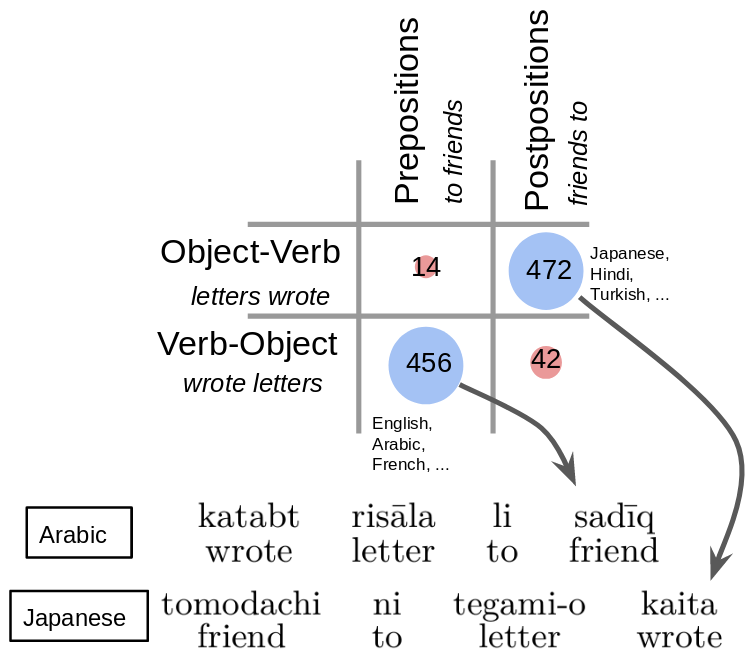
\includegraphics[width=0.4\textwidth]{figures/corr-full.png}
\caption{ One word order correlation: Languages can order the object after (Arabic) or before (Japanese) the verb, and have prepositions (Arabic) or postpositions (Japanese). For each combination, we indicate how many languages satisfy it, as documented in the World Atlas of Language Structures~\cite{wals}. Combinations on the diagonal are vastly more common than off-diagonal ones. 
	}\label{fig:arabic-japanese-simple}	\label{fig:corr-table}
\end{figure}



This generalization lies in a group of language universals originally documented by Greenberg \cite{greenberg1963universals}, known as \key{word order correlations}.
These describe correlations between the relative positions of different types of expressions across languages.
The example above documents that the position of the object (`letter') relative to the verb is \key{correlated} with the position of the adposition (`to'). %adpositional phrases (`to a friend') relative to the verb.
Greenberg also found that the order of verb and object is correlated with other aspects of a language's word order (Table~\ref{table:corr-dryer}), such the order of verb and adpositional phrase (`wrote -- to friend' in Arabic vs `friend to -- wrote' in Japanese), and that of noun and genitive (`book -- of friend' in Arabic, `friend of -- book' in Japanese).

\begin{table}[ht]
	\begin{center}
%		\setlength\tabcolsep{1.5pt}
\begin{tabular}{|c|ll|ll|}
	\hline
	%&
	&	\multicolumn{2}{c|}{\textbf{Arabic} (English, ...)}   &        \multicolumn{2}{c|}{\textbf{Japanese} (Turkish, ...)} \\ \hline\hline
	& \multicolumn{2}{c}{Correlates with...} & \multicolumn{2}{|c|}{Correlates with...}  \\
	&	Verb & Object     & Object & Verb    \\ \hline\hline
	& kataba & rasaa'il 	&tegami-o & kaita \\
	&	\emph{wrote} & \emph{letters} & 	\emph{letter} & \emph{wrote} \\ \hline 
	\multirow{2}{*}{\raisebox{.5pt}{\textcircled{\raisebox{-.9pt} {1}}}}	&	li    &    sadiiq       &	tomodachi & ni \\ % G3, G4
	&		\emph{to}            & \emph{a friend} &		\emph{friend} & \emph{to} \\ \hline 
	\multirow{2}{*}{\raisebox{.5pt}{\textcircled{\raisebox{-.9pt} {2}}}}	&kaana    &    sadiiq         &	tomodachi & datta \\ % not in Greenberg
	&	\emph{was}        & \emph{a friend} 	&\emph{friend} & \emph{was} \\ \hline
	\multirow{2}{*}{\raisebox{.5pt}{\textcircled{\raisebox{-.9pt} {3}}}}	&sawfa    &    yaktub       & 	kak & udesho \\ % G16, G13 TODO this should only be inflected auxiliaries, replace Arabic
	&	\emph{will}          & \emph{write}  &    	\emph{write} & \emph{will} \\ \hline
	\multirow{2}{*}{\raisebox{.5pt}{\textcircled{\raisebox{-.9pt} {4}}}}	& sadiiq  &    John    & 	John no & tomodachi \\ % G2, G23
	&	\emph{friend} &  \emph{of John}  &	\emph{John of} & \emph{friend} \\ \hline
	\multirow{2}{*}{\raisebox{.5pt}{\textcircled{\raisebox{-.9pt} {5}}}}	&kutub    &    taqra'uha       & 	anata-ga yonda & hon \\ % G24
	&	\emph{books} & \emph{that you read}  &	\emph{that you read} & \emph{book} \\ \hline
	\multirow{2}{*}{\raisebox{.5pt}{\textcircled{\raisebox{-.9pt} {6}}}}	&'an    &    tusil        & 	toochaku suru & koto \\ % 
	&	\emph{that} & \emph{she arrives}  &	\emph{has.arrived} & \emph{that} \\ \hline
	\multirow{2}{*}{	\raisebox{.5pt}{\textcircled{\raisebox{-.9pt} {7}}}}	&dhahabt	    &    'ila lmadrasa     & 	gakkoo ni & ittekimashita \\ % G22
	&	\emph{went} & \emph{to school}  &	\emph{school to} & \emph{went} \\ \hline
	\multirow{2}{*}{\raisebox{.5pt}{\textcircled{\raisebox{-.9pt} {8}}}}	&'uriid    &    'an 'ughaadir         & 	yom & itai \\ % G15
	& \emph{wants}   &  \emph{to leave}  &	\emph{to leave} & \emph{want} \\ \hline \hline
\end{tabular}
	\end{center}
	\caption{Greenberg's word order correlations, exemplified by Arabic (left) and Japanese (right) examples: Across the world, the orders of different constituents are strikingly correlated with that of verb and object.
	Selection is based on a more recent typological study by Dryer~\cite{dryer1992greenbergian}, restricted to those correlations that are annotated in available corpus data. See SI Section S1 for more on Greenberg correlations.
	}\label{table:corr-dryer}
\end{table}




Supported by languages on all continents, these correlations are among the language universals with the strongest empirical support.
Importantly, their validity is also independent from specific assumptions about theories of grammar.


Explaining these patterns has been an important aim of linguistic research since Greenberg's seminal study~\cite{lehmann1973structural, vennemann1974theoretical,jackendoff1977x,frazier1985syntactic,chomsky1988language, dryer1992greenbergian, hawkins1994performance}.
Prominent among this research is the argument that
%A prominent line of research has argued that 
language universals arise for \key{functional} reasons: that is, because they make human communication and language processing maximally efficient, and regularities across languages hold because these efficiency constraints are rooted in general principles of communication and cognition (e.g., \cite{gabelentz1901sprachwissenschaft,zipf1949human,hockett1960origin,pinker1990natural,givon1991markedness,hawkins1994performance,hawkins2004efficiency,hawkins2014crosslinguistic,croft2001functional,haspelmath2008parametric,jaeger2011language}).
Under this view, the various human languages represent multiple solutions to the problem of efficient information transfer given human cognitive constraints.

In an early and  influential functional framework,
Zipf \cite{zipf1949human} argued that language optimizes a tradeoff between two pressures: to reduce complexity and to reduce ambiguity.
%what he called the Forces of \emph{Unification} and %\emph{Diversification}.
What Zipf called the Force of Unification is a pressure to reduce the complexity of the language to make production and processing as easy as possible.
His Force of Diversification favors languages that provide different utterances for different meanings, so that the listener can unambiguously identify the meaning from the utterance.
These two forces act in opposing directions:
Producing and processing simple utterances incurs little cost, but more complex and diverse utterances are required  to provide enough information.
The idea that many properties of language arise from the tension between these two pressures has a long and fruitful history in linguistics~\cite{gabelentz1901sprachwissenschaft,horn1984toward, lindblom1990explaining, schwartz1997dispersion, hawkins2004efficiency, haspelmath2006against}.


Recent work has drawn on information theory  to computationally test this ``dual pressures'' idea in various domains of language, showing that it predicts
both basic statistical properties of languages~\cite{ferreri2003least} and language development~\cite{smith2013linguistic},
and sophisticated aspects of language, such as pragmatic inference \cite{frank2012predicting}, and the distribution of color words~\cite{zaslavsky2018efficient} and kinship categories~\cite{kemp2012kinship} across many languages.
While it has been suggested that the dual pressure  should also apply to grammar~\cite{hawkins2004efficiency}, testing these accounts is more difficult, as this requires  large amounts of data representative of language use across languages,  computational methods for estimating the efficiency of entire languages, and a simulation methodology for comparing different possible grammars.

In this work, we address these challenges by combining large-scale text data from 51 languages with machine learning techniques to estimate both aspects of the communicative efficiency of grammar: complexity and ambiguity.
We use machine learning models based on neural networks to model the evolution of grammars towards efficiency.
We apply this approach to the problem of explaining Greenberg's word order correlation universals.

In Study 1 we compare the word order of actual grammars of 51 languages with alternative ``counterfactual'' grammars parameterized by different word orders. We use our model to measure the communicative efficiency of each possible grammar, showing  that the grammars of real languages are more efficient than alternative  grammars. The fact that real grammars lie at the Pareto frontier of the efficiency space of possible  grammars suggests that the word order of languages has evolved to optimize communicative efficiency.

In Study 2 we test whether efficiency optimization accounts for the Greenbergian word order correlations.  For each of the 51 languages, we create hypothetical grammars optimized for efficiency.  We then test statistically whether these optimized grammars exhibit the Greenberg correlations, using a Bayesian mixed-effects logistic regression to control for language and language family.  Efficiency optimization indeed predicts all eight Greenberg collections.
%
%and makes fine-grained per-language predictions about individual syntactic patterns.
Our results show how general properties of efficient communication give rise to these universal word order properties of human language.







%\section*{Paradigm:   Random Grammars}
%
%In order to test whether 

%idea of counterfactual grammars.  hypothetical grammars with different orders, so can study properties.

%\begin{figure}[ht]
%    \centering
%    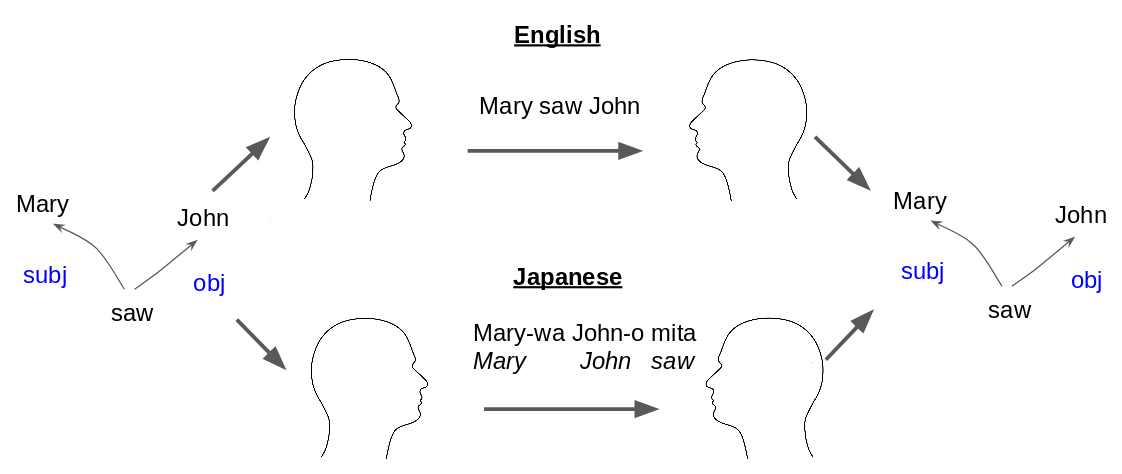
\includegraphics[width=0.45\textwidth]{figures/communication-two-langs.png}
%	\caption{Grammars define cAommunication channels: A speaker (left) expresses a syntactic structure into a string of words forming a sentence. The order of words is determined by the grammar of the language. A listener recovers a syntactic structure. Communication is successful if the listener recovers the correct depenency structure.}
%	\label{fig:comm}
%\end{figure}










%We model the process where a speaker communicates a message to a listener (Figure~\ref{fig:comm}) in Shannon's framework of information theory.
%In this model, a transmitter encodes a message into a signal. The receiver decodes the signal, attempting to reconstruct the original message.
%Applying this model to word order, we take the message to consist of people, objects, events, and a set of syntactic and semantic relations that hold between them~\cite{fodor1975language,jackendoff1983semantics,pinker1990natural}.


%TODO also need to mention Principle of Compositionality, as additional justification for why listener needs to recover syntactic structures


%Consider Figure~\ref{fig:comm}.
%Imagine the speaker wants to communicate that Mary saw John.
%The message (left) consists of a syntactic structure with the words `saw', `Mary', `John', where Mary is the subject of the event denoted by `saw', and John is the object.
%When uttering, the speaker needs to choose an ordering in which to order the words in this tree to generate a string of words.
%In human language, this order is largely determined by the \key{grammar} of the language (CITE).
%The speaker will order it as \emph{Mary saw John} (Figure~\ref{fig:comm}, top) in English, and as \emph{Mary John saw} (Figure~\ref{fig:comm}, bottom) in Japanese.
%The listener receives a sentence -- a linear string of words -- and decodes the underlying message in accordance with the grammar of the language (Figure~\ref{fig:comm}, right).





\section*{Grammars and Grammar Data}

Following a long tradition in theoretical and computational linguistics, we formalize  the grammatical structure of languages using dependency trees~\cite{hays1964dependency,melcuk1988dependency,corbett1993heads,tesniere2015elements}.
%This linguistic formalism draws directed arcs between syntactically related words, annotated with grammatical relations like subject or object.
This linguistic formalism represents grammatical dependencies as directed arcs between syntactically related words, annotated with grammatical relations like subject or object (Figure~\ref{fig:sent-dep}).
While syntactic formalisms vary, the dependency grammar community has an agreed representation format  which has been used to  annotate corpora of text from dozens of languages \cite{ud2.1}, and there are 
computational methods for mapping syntactic structures in this representation to other standard linguistic formalisms \cite{boston2009dependency}.

\begin{figure}[ht]
    \centering
{
\centering{
\begin{dependency}[theme = simple]
   \begin{deptext}[column sep=1em]
          She \& met \& friends  \\
   \end{deptext}
        %   \deproot{3}{ROOT}
   \depedge{2}{1}{subject}
   \depedge{2}{3}{object}
   %\depedge[arc angle=50]{7}{6}{ATT}
\end{dependency}
}
}
	\caption{An English sentence with annotated syntactic relations.}
	\label{fig:sent-dep}
\end{figure}

Our models require a sample of  syntactic structures as actually used by speakers across different languages, for which we draw on the recent
Universal Dependencies project~\cite{ud2.1}, which has collected and created syntactic annotations for several dozens of different languages.
51 languages had sufficient data for our purposes. 
These corpora represent a typologically and genetically diverse group of languages. %  (see Figure~\ref{fig:per-lang})
We obtained a total of 11.7M words in 700K sentences annotated with syntactic structures; with a median of 117K words and 7K sentences for each individual language.



\section*{Study 1: Relative efficiency of languages}
\label{sec:relative-efficiency}

We first ask whether the grammars of human languages evolve towards optimizing efficiency of communication.  To do this we
%We first demonstrate that the grammars of real languages are relatively efficient compared to random baselines, providing evidence that grammars evolve towards efficiency.
compare the efficiency of the actual grammars of the 51 languages from the Universal Dependencies datasets to randomly constructed baseline grammars.
 

The grammars of natural languages specify how the different words in a syntactic structure are ordered into a sentence, i.e., a string of words  \cite{adger2015syntax}.
%Grammars do this largely by providing consistent ordering rules for all syntactic relations (such as subjects and objects).
This is illustrated in Figure~\ref{fig:grammars}:
We show how four different grammars order objects, adpositional phrases, and adpositions.
For instance, Grammar 1 -- corresponding to Arabic in Figure~\ref{fig:arabic-japanese-simple} -- orders objects (`friends', `letter') after verbs and has prepositions (`to friend').
Grammar 2 orders objects after verbs but has postpositions (`friend -- to').
Grammars 3 and 4 place the object before the verb, and one of them (Grammar 3) corresponds to Japanese order.
%Grammars 2 and 4 are rare or impossible.

\begin{figure}[ht]
    \centering
    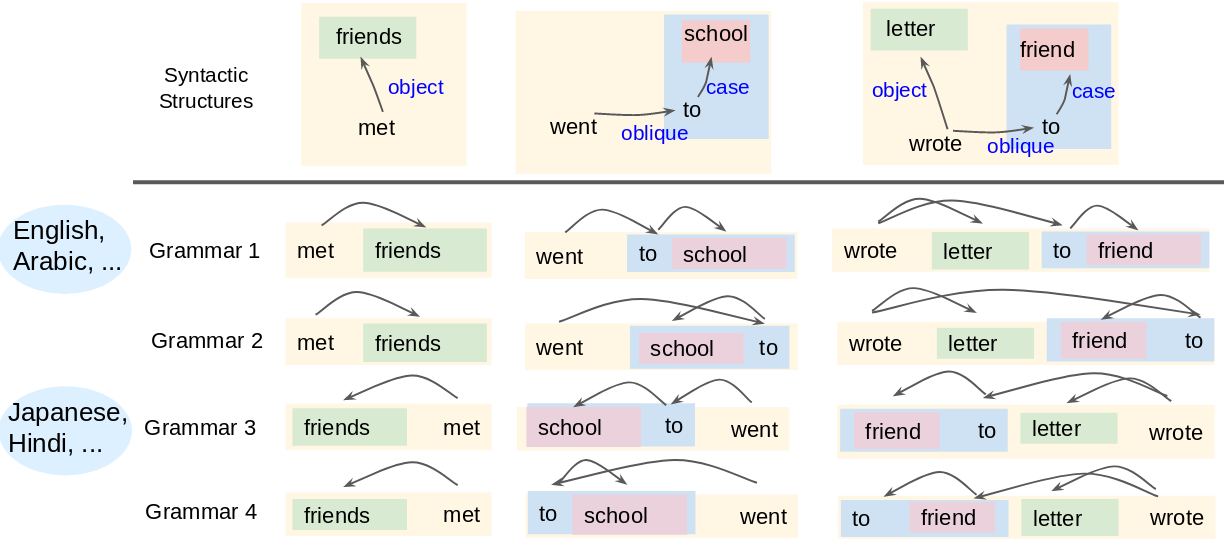
\includegraphics[width=0.48\textwidth]{figures/grammar-langs-fontsize-friends.png}
	\caption{Grammars define consistent ordering rules for syntactic structures. Here, Grammars 1 and 2 order the object after the verb, Grammars 3 and 4 order the object before the verb. Grammars 1 and 3 conform to the Greenberg correlations and are common around the world; Grammars 2 and 4 are rare or impossible.}
	\label{fig:grammars}
\end{figure}

Beyond the syntactic relations exemplified in Figure~\ref{fig:grammars}, human languages have further types of syntactic relations.
The Universal Dependencies project, the source of our data, defines a total of 38 syntactic relations.
We adopt the grammar model of Gildea and colleagues~\cite{gildea2007optimizing, gildea2010grammars, gildea2015human}; a grammar assigns a weight from $[-1,1]$ to each of these 38 syntactic relations, and orders words according to the weights assigned to their relations
%Words that are syntactic dependents of the same word are ordered according to the weights assigned to the syntactic relations that link each of them to that word 
(See \textit{Materials and Methods} for details).

Given a database of syntactic structures (such as those at the top of Figure~\ref{fig:grammars}), obtained from a corpus of some real language L , we can apply a grammar to order the structures in the database into a dataset of counterfactual sentences belonging to a hypothetical language defined by that grammar (Figure~\ref{fig:grammars}).
This hypothetical language has identical syntactic structures and grammatical relations as the true language L, but different word order.

We create baseline grammars by randomly sampling the weights for each syntactic relation.
These baseline grammars have systematic word order rules similar to natural language, but do not exhibit any correlations among the orderings of different syntactic relations.
All four grammars in Figure~\ref{fig:grammars} are equally likely under this baseline distribution.

%For a language L, we obtain counterfactual versions 

%Each of these random grammars for a language L has the identical syntactic structure and grammatical relations as the true grammar of L, but have different word orders.  

%We therefore built a minigrammar for each language L with the same syntactic structures but with different orderings.

For every one of the 51 languages, we construct 50 counterfactual versions by randomly creating 50 baseline grammars, applying these to obtain counterfactual orderings for all syntactic structures that were available for that language.
%Each grammar specifies a weight from [-1,1] to each of these 38 syntactic relations.
%Words that are syntactically related to the same word are ordered according to these weights \cite{gildea2007optimizing}.


Following the information-theoretical literature on language processing, 
we formalize the  efficiency of a language as a weighted combination of two terms:  the 
amount of information that utterances contain about the underlying messages, and the  cost or difficulty of communication~\cite{ferreri2003least,frank2012predicting,zaslavsky2018efficient,kemp2012kinship,regier2015word,goodman2013knowledge}.
We model the informativity term as the 
 degree to which listeners can reconstruct syntactic structures from an utterance, i.e., the \key{parseability} of the language. We model the cost or complexity term as the 
 \key{predictability}, or negative entropy, of the utterances. %, since entropy is a standard measure of the complexity of any message.
 We then estimate predictability and parseability using standard neural network models, and combine them linearly to produce a single model for efficiency.
 See \textit{Materials and Methods} for details.

For every one of the 51 languages, we computationally construct grammars that are \emph{optimized} for parseability, predictability, and efficiency (see \textit{Materials and Methods}).
This optimization problem is challenging because both the parseability and predictability of a sentence can only evaluated globally, in the context of an entire language.
We address this challenge by using neural network methods to estimate parseability and predictability, and by introducing a simple, differentiable computational formalism for describing grammatical regularities. 
This setup means that it is possible to find optimal grammars by standard methods such as stochastic gradient descent (see SI section S5).
For each grammar, we report predictability and parseability as estimated on the data resulting from ordering the syntactic structures from the corpus according to the grammar.


\begin{figure}
    \centering
    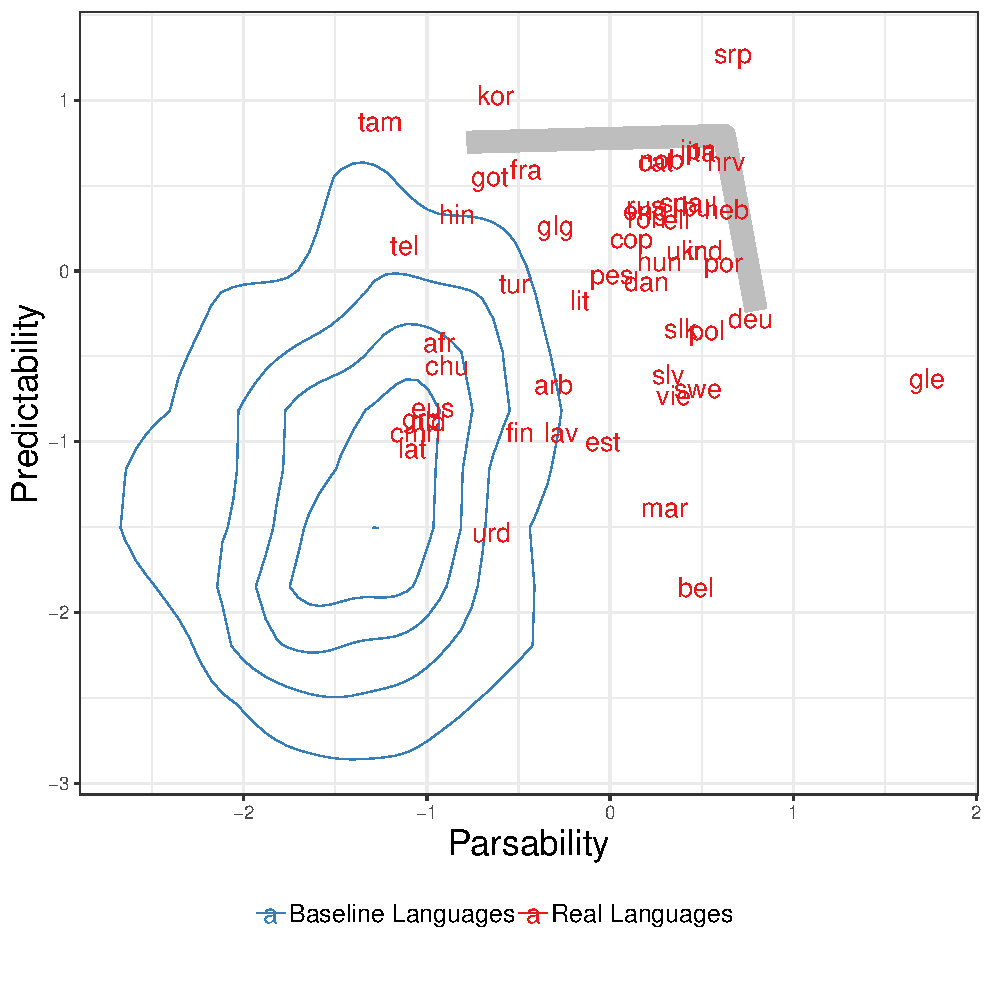
\includegraphics[scale=.5]{../results/plane/pareto-plane-iso-best-balanced-legend-viz-10-fontsize.pdf} % mention how many independent N's there are?
    \caption{Predictability and parseability of 51 languages (red), indicated by ISO codes, compared to baseline word order grammars (blue distribution). Predictability and parseability scores are $z$-scored within language. The gray curve indicates the Pareto frontier of computationally optimized grammars, averaged over the 51 languages.} 
    \label{fig:pareto-plane}
\end{figure}

In Figure~\ref{fig:pareto-plane}, we plot predictability and parseability of the grammars of 51 languages, together with the distribution of random baseline grammars, and the Pareto frontier defined by computationally optimized grammars.
Languages are attracted towards the Pareto frontier and away from the region of the baseline languages.
The majority of real languages are above and to the right of their baseline equivalents, demonstrating that they are relatively high in predictability and/or parseability.
100~\% of languages improve on either predictability or parseability ($p<0.05$, by one-sided $t$-test, with Bonferroni correction and Hochberg's step-up procedure \cite{hochberg1988sharper}).
90~\% of languages improve over the baselines in parseability ($p < 0.05$), 80~\% improve in predictability ($p < 0.05$).
See SI Section S3 for additional analyses.




\section*{Study 2: Greenberg Word Order Correlations}
\label{sec:greenberg}

%\begin{figure} 
%	\begin{center}
%	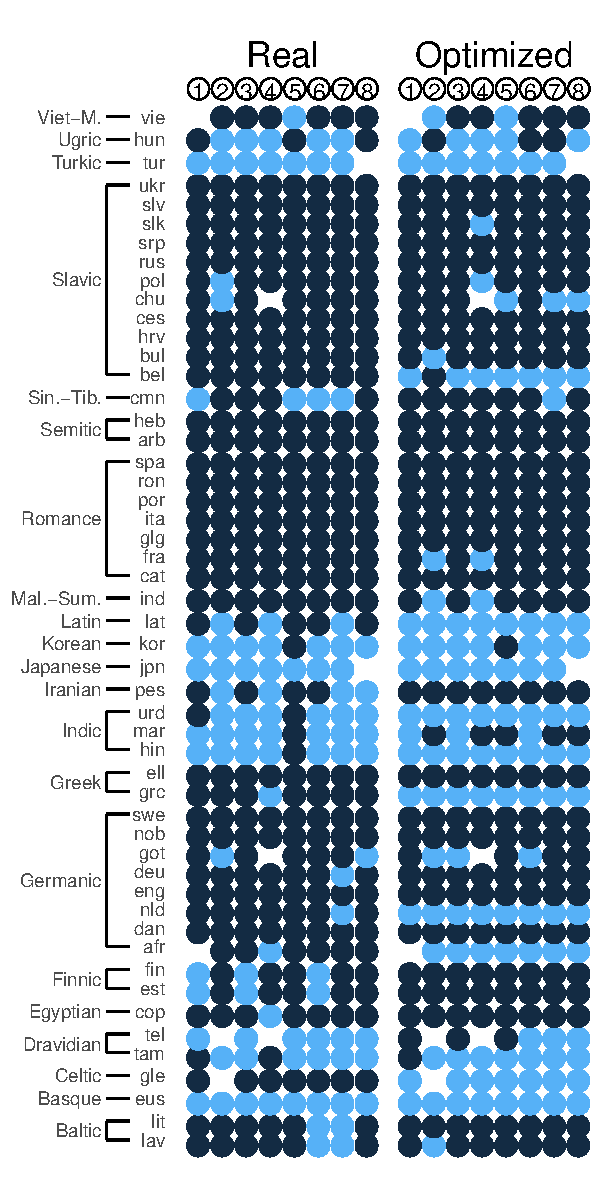
\includegraphics[width=0.32\textwidth]{../results/correlations/figures/pred-eff-families-2.pdf}
%	\end{center}
%	\caption{Order of the eight correlates across 51 languages, in the real grammars (left) and predicted by efficiency optimization (right). Dark blue: Verb patterner \emph{precedes} object patterner(English, Arabic, ...). Light blue: Verb patterner \emph{follows} object patterner (Japanese, Hindi , ...).}\label{fig:per-lang}
%\end{figure}




We have found that the grammars of human languages concentrate along the Pareto frontier of parseability and predictability.
This does not yet, however, say anything about what grammatical properties characterize Pareto-optimal languages in general, or which properties of human languages make them efficient.



We show that all languages close to the Pareto frontier -- both real and counterfactual ones -- are highly likely to satisfy Greenberg's correlation universals.
That is, optimizing for efficiency produces languages that satisfy these correlations.
In contrast, the baseline grammars are constructed without any correlations between the ordering of different syntactic relations, and will therefore not satisfy any of those universals.

We first considered this question for the 51 real languages.
Among the real grammars of the 51 languages, the number of satisfied correlations is strongly correlated with efficiency ($\rho = 0.61$, $p<0.0001$). %, and also with parseability ($\rho = 0.57$, $p<0.0001$) and predictability ($\rho =0.33$, $p = 0.024$) individually.
%(Parseability and predictability were $z$-scored within language as in Figure~\ref{fig:pareto-plane}. \textcolor{red}{TODO})


We next examine those grammars from Study 1 that we had computationally optimized for efficiency.
We controlled for variation across different optima by creating eight optimized grammars for each of the 51 datasets of syntactic structures from real languages.
For each language, we created four grammars with verb-object order, and four object-verb grammars.
We test whether the process of efficiency optimization produces the Greenberg correlations.


For each grammar (baseline, optimized, and real), we computed how many of the eight relations in Table~\ref{table:corr-dryer} had the same order as  Japanese (in contrast to Arabic).
Figure~\ref{fig:joint} shows the results, separately for grammars with verb-object and object-verb orders.
In optimized grammars, the order of the eight relations is strongly correlated with the placement of the object, similar to the 51 real languages in our sample.
In contrast, baseline languages show no correlation.


\begin{figure}
    \centering
    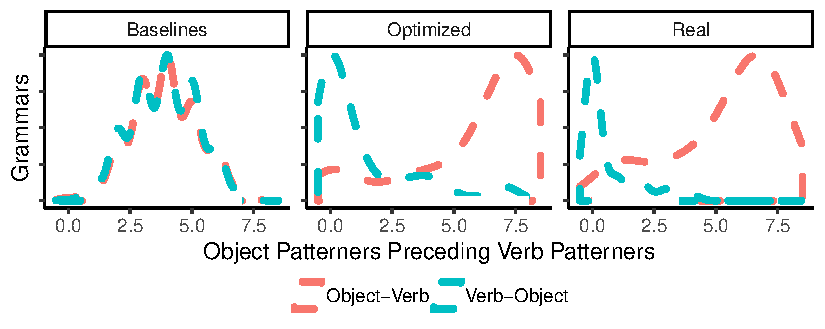
\includegraphics[width=0.48\textwidth]{../results/correlations/figures/correlations-curve-whiteaxis.pdf}
    %{figures/joint-results-corrs-curves.png} % ~/grammar-optim/results/correlations/figures/correlations-curve.pdf
    \caption{
    Efficiency optimization produces grammars where the orders of the eight relations in Table~\ref{table:corr-dryer} are strongly correlated with the order of verb and object. We arrange grammars (baseline, optimized, real) by the number of relations where the language patterns with Japanese (as opposed to with Arabic), and plot a kernel density estimate. Object-Verb order leads to grammars where object patterners precede (like Japanese); verb-object order leads to verb patterners preceding (like Arabic). Baseline grammars show no such correlation.
    }
    \label{fig:joint}
\end{figure}



%We compare grammars optimized for efficiency with the actual grammars of the 51 languages, as extracted from the orderings attested in the original corpora and validated against expert judgments (see \textit{Materials and Methods}).

So far, our results show that languages are efficient in part because they mostly satisfy the Greenberg correlations.
We asked whether efficiency optimization predicts every one of the eight correlations to hold in most languages.
We constructed a Bayesian multivariate logistic regression model predicting which of the eight correlations an optimized grammar satisfies.
%We first evaluated which of the eight correlations emerge from efficiency optimization across language families.
We controlled for variation between the syntactic structures used in different languages and language families by entering the language and language family as random effects.
See SI Section S4.3 for details.




\begin{table}
	\begin{center}
\begin{tabular}{|c|ll|c|cc|ccc}
	\hline
	%&
	&	\multicolumn{2}{c|}{Correlates with...}   &         \multirow{2}{*}{Real}   &  \multirow{2}{*}{Optimized} & \\ 
	&	verb & object     & & &   \\ 
	&	\emph{wrote} & \emph{letters} & & & \\ \hline \hline 
	\multirow{2}{*}{\raisebox{.5pt}{\textcircled{\raisebox{-.9pt} {1}}}}	&	adposition    &    NP       
				&   \multirow{2}{*}{  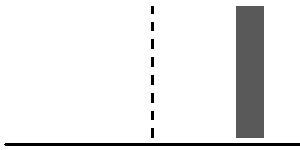
\includegraphics[width=0.06\textwidth]{../results/correlations/figures/posteriors/posterior_Real_lifted_case.pdf}     } 
		&   \multirow{2}{*}{  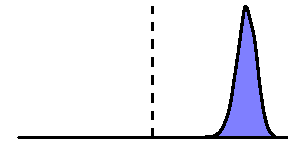
\includegraphics[width=0.06\textwidth]{../results/correlations/figures/posteriors/posterior_Efficiency_lifted_case.pdf}     } & \\
	&		\emph{to}            & \emph{a friend} &&&\\ \hline
	\multirow{2}{*}{\raisebox{.5pt}{\textcircled{\raisebox{-.9pt} {2}}}}	&copula    &    NP         
		&   \multirow{2}{*}{  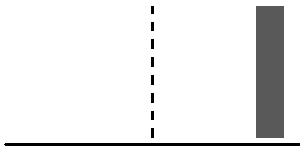
\includegraphics[width=0.06\textwidth]{../results/correlations/figures/posteriors/posterior_Real_lifted_cop.pdf}     } 
		&   \multirow{2}{*}{  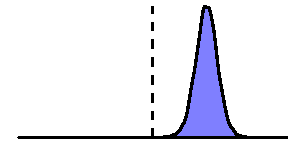
\includegraphics[width=0.06\textwidth]{../results/correlations/figures/posteriors/posterior_Efficiency_lifted_cop.pdf}     } & \\
	&	\emph{is}        & \emph{a friend}  &&&\\ \hline
	\multirow{2}{*}{\raisebox{.5pt}{\textcircled{\raisebox{-.9pt} {3}}}}	&auxiliary    &    VP       
		&   \multirow{2}{*}{  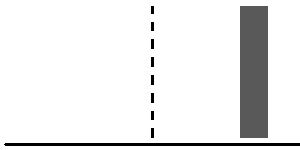
\includegraphics[width=0.06\textwidth]{../results/correlations/figures/posteriors/posterior_Real_aux.pdf}     } 
		&   \multirow{2}{*}{  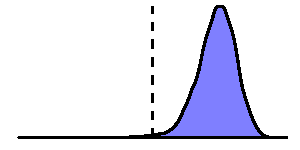
\includegraphics[width=0.06\textwidth]{../results/correlations/figures/posteriors/posterior_Efficiency_aux.pdf}     } & \\
	&	\emph{has}          & \emph{written}  &&&\\ \hline
	\multirow{2}{*}{\raisebox{.5pt}{\textcircled{\raisebox{-.9pt} {4}}}}	&noun    &    genitive      
		&   \multirow{2}{*}{  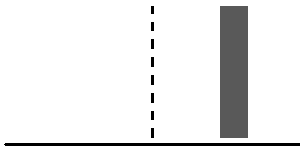
\includegraphics[width=0.06\textwidth]{../results/correlations/figures/posteriors/posterior_Real_nmod.pdf}     } 
		&   \multirow{2}{*}{  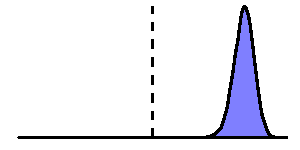
\includegraphics[width=0.06\textwidth]{../results/correlations/figures/posteriors/posterior_Efficiency_nmod.pdf}     } & \\
	&	\emph{friend} &  \emph{of John}  &&&\\ \hline
	\multirow{2}{*}{\raisebox{.5pt}{\textcircled{\raisebox{-.9pt} {5}}}}	&noun    &    relative clause      
		&   \multirow{2}{*}{  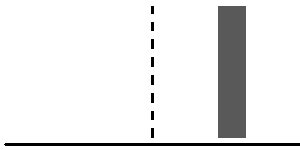
\includegraphics[width=0.06\textwidth]{../results/correlations/figures/posteriors/posterior_Real_acl.pdf}     } 
		&   \multirow{2}{*}{  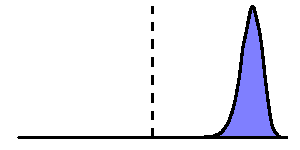
\includegraphics[width=0.06\textwidth]{../results/correlations/figures/posteriors/posterior_Efficiency_acl.pdf}     } & \\
	&	\emph{books} & \emph{that you read}  &&&\\ \hline
	\multirow{2}{*}{\raisebox{.5pt}{\textcircled{\raisebox{-.9pt} {6}}}}	&complementizer    &    S        
		&   \multirow{2}{*}{  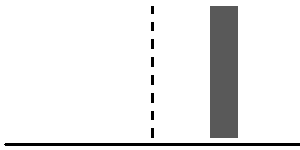
\includegraphics[width=0.06\textwidth]{../results/correlations/figures/posteriors/posterior_Real_lifted_mark.pdf}     } 
		&   \multirow{2}{*}{  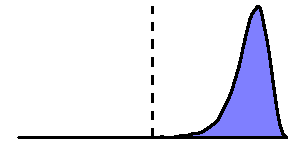
\includegraphics[width=0.06\textwidth]{../results/correlations/figures/posteriors/posterior_Efficiency_lifted_mark.pdf}     } & \\
	&	\emph{that} & \emph{she has arrived}  &&&\\ \hline
	\multirow{2}{*}{	\raisebox{.5pt}{\textcircled{\raisebox{-.9pt} {7}}}}	&verb    &    PP         
		&   \multirow{2}{*}{  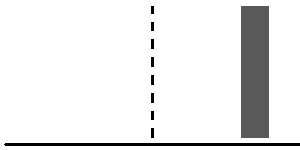
\includegraphics[width=0.06\textwidth]{../results/correlations/figures/posteriors/posterior_Real_obl.pdf}     } 
		&   \multirow{2}{*}{  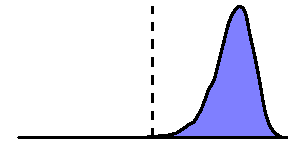
\includegraphics[width=0.06\textwidth]{../results/correlations/figures/posteriors/posterior_Efficiency_obl.pdf}     } & \\
	&	\emph{went} & \emph{to school}  &&&\\ \hline
	\multirow{2}{*}{\raisebox{.5pt}{\textcircled{\raisebox{-.9pt} {8}}}}	&want    &    VP        
		&   \multirow{2}{*}{  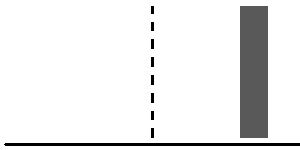
\includegraphics[width=0.06\textwidth]{../results/correlations/figures/posteriors/posterior_Real_xcomp.pdf}     } 
		&   \multirow{2}{*}{  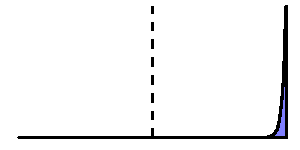
\includegraphics[width=0.06\textwidth]{../results/correlations/figures/posteriors/posterior_Efficiency_xcomp.pdf}     } & \\
	& \emph{wants}   &  \emph{to leave}  &&&\\ \hline
 \hline
\end{tabular}
	\end{center}
\caption{Efficiency optimization accurately predicts the Greenbergian correlations.
For each correlation, we provide the prevalence among the actual grammars of the 51 languages (left), and the posterior distribution of the prevalence among grammars optimized for efficiency (right).
Efficiency optimization predicts all eight correlations to hold in the majority of grammars. \textcolor{red}{make visually clear that it's 51 languages}
}\label{table:corr-resu}
\end{table}




In Table~\ref{table:corr-resu}, we compare the prevalence of the eight correlations in real and optimized languages.
For the real languages, we indicate how many of the 51 languages satisfy a correlation.
For the optimized languages, we indicate the posterior distribution of the proportion of satisfying languages, obtained from the mixed-effects analysis. % (see \textit{Materials and Methods}).
Grammars optimized for efficiency accurately predict all eight correlations to hold at prevalences significantly greater than 50\%, similar to actual human languages.
In the multivariate mixed-effects analysis, efficiency optimization predicts all eight correlations to hold across languages (posterior probability $0.9911$). 
Optimizing for only predicability or only parseability does not predict all of the correlations (See SI Section S4.4).




%We confirmed these results by evaluating predictions of efficiency optimization on the level of individual languages (Figure~\ref{fig:per-lang}).
%For every one of the 51 languages, we show orders predicted by efficiency, for the eight correlating pairs.
%For each language, we consider the optimized grammar that had the best efficiency value, among those with the direction of the verb-object relation fixed to correspond to the actual language.
%Predictions of efficiency optimization agree with the actual word order patterns in 82~\% of the cases.
%Note that perfect agreement is not to be expected, as grammars will be impacted by factors other than efficiency optimization, such as their historical development.
%For instance, Dutch (nld) and Afrikaans (afr) have a prevalence of object-verb order in corpus data, and efficiency optimization accordingly predicts them to have corresponding orders (light blue).
%However, Dutch and Afrikaans have orders similar to the other Germanic languages (dark blue), which they are historically closely related to.






%We have directly implemented parseability and predictability using general-purpose statistical models of language and syntactic structures.
%Prior work has considered Dependency Length Minimization (DLM) as an approximate formalization of efficiency optimization~\cite{futrell2015largescale,liu2017dependency,temperley2018minimizing}.
%This is the idea that languages order words so as to minimize the overall length of syntactic relations.
%This principle is a heuristic formalization of the idea that long syntactic relations should create high memory requirements in parsing and prediction~\cite{hawkins1994performance,gibson1998linguistic,gibson2000dependency, futrell2017memory}.
%Indeed, directly modeling efficiency optimization predicts DLM, and appears to predict word order universals with greater accuracy than optimizing for DLM (see  \emph{Relation to Dependency Length Minimization}).



\section*{Discussion}

We found that the grammars of natural languages are more efficient than baseline grammars, and that a large subset of the Greenbergian word order correlations can be explained in terms of optimization of grammars for efficient communication. %, as defined by information theoretic criteria and implemented using state-of-the-art machine learning methods.
%\textcolor{red}{[TODO adapt the next sentence to framing]} %We defined a space of word order grammars, as well as objective functions reflecting communicative efficiency, and found that the word order grammars that maximize communicative efficiency reproduce the word order universals. 


Our work makes crucial use of neural network models for estimating the efficiency of languages.
This method currently requires large computational resources; it still takes about three weeks to create optimized grammars for 51 languages, even with specialized hardware.
We believe that further advances in machine learning will reduce the computational cost, making this approach more widely applicable.

%This is the idea that languages order words so as to minimize the overall length of syntactic relations.
%This principle is a heuristic formalization of the idea that long syntactic relations should create high memory requirements in parsing and prediction~\cite{hawkins1994performance,gibson1998linguistic,gibson2000dependency, futrell2017memory}.

What makes the grammars of human languages efficient?
Study 2 shows that Greenberg's correlations are one key property that real languages share with optimal grammars.
Prior work has suggested \emph{Dependency Length Minimization} as another characteristic of efficient word order.
This is the idea that word order minimizes the average distance between syntactically related words.
%Prior work has suggested some other properties as characteristics of efficient word order.
%One such property is Dependency Length Minimization, the idea that word order minimizes the distance between syntactically related words.
It is known that human languages reduce this distance compared to random baselines~\cite{futrell2015largescale,liu2017dependency,temperley2018minimizing}.
Indeed, 100\% of grammars optimized for efficiency also reduce average distance between related words  compared to baselines ($p < 0.05$, by one-sided $t$-test).
To some extent, the Greenberg correlations help reduce the distance between related words. Consider again the sentence `I wrote letters to friends' (cf. Figures~\ref{fig:corr-table} and \ref{fig:grammars}). Both real and optimized grammars of English linearize its syntactic structure as follows:
\begin{center}
\begin{dependency}[theme = simple]
   \begin{deptext}[column sep=1em]
          I \& wrote \& letters \& to \& friends  \\
   \end{deptext}
        %   \deproot{3}{ROOT}
   \depedge{2}{1}{subject}
   \depedge{2}{3}{object}
   \depedge{2}{4}{oblique}
   \depedge{4}{5}{case}
   %\depedge[arc angle=50]{7}{6}{ATT}
\end{dependency}
\end{center}
Note that this ordering exhibits correlations (1) and (7) from Table~\ref{table:corr-dryer}.
Among all possible ways of ordering this syntactic structure, this ordering also minimizes the average distance between any two syntactically related words: E.g., inverting `to' and `friends' would increase the distance between `wrote' and `to'.
%\textcolor{red}{I'm thinking about removing this part, I think it's a bit close to giving away the main result of another paper.}
%\textcolor{orange}{A second suggested property of efficient word order is Information Locality~\cite{gildea2015human,futrell2017noisycontext}, the idea that words that predict each other should be close.
%94~\% of the real grammars, and 90~\% of optimized grammars have significantly higher degrees of information locality than baseline grammars (at $p < 0.05$, one-sided $t$-test).}
Understanding mathematically why dependency length minimization  improves efficiency is an important problem for future research.
%and information locality


%\textcolor{red}{TODO revise this and make this about simplicity of the grammar, also harmonize with succeeding paragraph}
An idea related to, but distinct from, functional optimization is the idea that grammars are biased towards simplicity \cite{smith2013linguistic}. %\textcolor{red}{(TODO what to CITE here)} 
It has been proposed that languages have a single head-directionality parameter and that this accounts for the Greenberg correlations \cite{chomsky1988language}.
%We note that, for the eight syntactic relations in Table~\ref{table:corr-dryer}, the element patterning with the verb is often classified as the \emph{head} of the relation in syntactic theories.
%One way to capture the generalization would have been to stipulate that language has a single head directionality parameter, and assume that languages have identical head direction across different syntactic relations.
As an explanation of correlations, this idea makes strong predictions, and turns out to overpredict correlations \cite{dryer1992greenbergian}.
Nevertheless, future research should examine whether there are more principled connections between communicative efficiency and grammar simplicity.
%Our results, however, show that the tendency towards consistent head directionality is explainable from communicative principles.




A major question for functional explanations for linguistic universals is: \emph{how} do languages end up optimized? Do speakers actively seek out new communicative conventions that allow better efficiency? Or do languages change in response to biases that come into play during language acquisition \cite{fedzechkina2012language,culbertson2012learning}? Our work is neutral toward such questions. To the extent that language universals arise from biases in learning or in the representational capacity of the human brain, our results suggest that those biases tilt toward communicative efficiency. Our work does provide evidence against the idea that word order universals are best explained in terms of learning biases that are irreducibly arbitrary and genetic in nature \cite{chomsky2010some}.

While our work has shown that certain word order universals can be explained by efficiency in communication, we have made a number of basic assumptions about how language works in constructing our word order grammars: for example, that sentences can be syntactically analyzed into trees of syntactic relations. The question arises of whether these more basic properties themselves might be explainable in terms of efficient communication.


%\textcolor{red}{TODO unify the next two paragraphs}
Beyond those universals that we examined, Greenberg~\cite{greenberg1963universals} described other universals; some of those are syntactic and could be tested with more specific annotation of datasets; others are not syntactic and are beyond the scope of this study.
Beyond Greenberg's work, there are remaining word order universals not captured by our model, such as the trade-off of rich morphological marking and flexibility in word order \cite{jespersen1922,mcfadden2003morphological,futrell2015quantifying}.
Our models do not capture this trade-off because the grammar model assumes fixed word order.
Future work can investigate whether these and other remaining universals can be explained using more sophisticated models of how syntactic structures are transduced into strings of words, based on larger databases with richer annotations.


These questions notwithstanding, our work provides strong evidence that the grammatical structure of languages is shaped by the need to support efficient communication.
Beyond our present results, we provide a computational framework in which theories of the efficiency optimization of languages can be tested.
While our study has focused on syntax, our results suggest that this method can be fruitfully applied to testing efficiency explanations in other domains of language structure.
%Despite to date only syntax, ...
%Other objective functions could be hypothesized and tested within our framework
%Furthermore, future advances in machine learning will enable the optimization of richer and richer models of grammar.

\matmethods{
\unskip
\subsection*{Corpus Data}
We base our experiments on the Universal Dependencies 2.1 treebanks~\cite{ud2.1}. % \footnote{\url{http://universaldependencies.org/}}
We use all languages for which at least one treebank with a training partition was available, a total of 51 languages.
For each language where multiple treebanks with training sets were available, we pooled their training sets; similarly for development sets.
Punctuation was removed.

%Universal dependencies deviates from standard syntactic theory in the representation of certain syntactic relations.
Universal dependencies represents as dependents some words that are typically classified as heads in syntactic theory.
This particularly applies to the \textit{cc}, \textit{case}, \textit{cop}, and \textit{mark} dependencies.
Following prior work studying dependency length minimization \cite{futrell2015largescale}, we applied automated conversion to a more standard formalism, modifying each treebank by inverting these dependencies, and promoting the dependent to the head position.
%We report results on this modified version of UD.

\subsection*{Word Order Grammars}
We adapt the grammar model of~\cite{gildea2007optimizing} to UD.
A grammar assigns a parameter $x_\tau \in [-1,1]$ to every relation  $\tau$ belonging to the 38 universal syntactic relations defined by UD.
A syntactic structure, consisting of a set of words and syntactic relations between them, is then ordered into a string of words recursively starting from the root; the dependents of a word then are ordered around the head according to the values $x_\tau$ corresponding to their syntactic relations; those dependents where $x_\tau < 0$ are ordered before the head; the others after the head.
See SI Section S5.2 for the methodology used to extract the languages' actual grammars from datasets, and for validation against expert judgments.

\subsection*{Formalizing Efficiency}
We adopt the formalization of language efficiency of \cite{ferreri2003least}, equivalent to a deterministic version of the Information Bottleneck \cite{zaslavsky2018efficient}.
Very similar formalizations of Zipf's ideas have been proposed across the information-theoretic literature on language~\cite{frank2012predicting,kemp2012kinship,regier2015word}. 
See SI Section S2 for discussion.
%The efficiency of any information-theoretic communication protocol depends on (1) how costly encoding and transmission are, and (2) how precisely messages can be recovered from codes~\cite{shannon1948mathematical}.
% both information theory~\cite{shannon1948mathematical}, and
%Following prior computational studies of functional explanations in linguistics~\cite{ferreri2003least,frank2012predicting,zaslavsky2018efficient,kemp2012kinship,regier2015word,goodman2013knowledge}, 

In this framework, the overall efficiency of language is a weighted combination of terms representing the amount of information that utterances contain about the underlying messages, and the cost of communication  \cite{ferreri2003least,frank2012predicting,kemp2012kinship,regier2015word,zaslavsky2018efficient}. We model the first term as the 
 degree to which listeners can reconstruct syntactic structures from an utterance, i.e., the \key{parseability} if the language.
 This is formalized as the amount of information that utterances $u$ provide about their underlying syntactic structures $t$:
\begin{equation}
	R_{Pars} := I[\mathcal{U},\mathcal{T}] = \sum_{t,u} p(t,u) \log \frac{p(t|u)}{p(t)}
\end{equation}
where the sum runs over all possible pairs of utterances $u$ and syntactic structures $t$ in the language.
%This quantity describes the degree to which syntactic structures can be unambiguously recovered from sentences, and quantifies how successful communication is (cf. Figure~\ref{fig:comm}).

Again following \cite{ferreri2003least}, we formalize the complexity of a language as its entropy~\cite{ferreri2003least,ferrericancho2007global,futrell2017memory}.
This corresponds to the average word-by-word surprisal, the degree to which sentences are unpredictable from the general statistics of the language.
Surprisal has been found to be a highly accurate and general predictor of human online processing difficulty \cite{hale2001probabilistic,levy2008expectation,smith2013effect}.
%and can be justified  in terms of predictive coding theories of information processing in the brain \cite{friston2009predictive} as well as the general algorithmic complexity of language generation and comprehension \cite{li2008introduction}.
In expectation over all utterances $u$ in a language, the negative surprisal describes the \key{predictability}, or negative entropy, of the utterances:
\begin{equation}
	R_{Pred} := - H[\mathcal{U}] = \sum_{u} p(u) \log p(u)
\end{equation}
where the sum runs over all possible sentences $u$ that belong to the language.
%In keeping with Zipf's Force of Unification, this quantity describes how homogeneous the language is, i.e., it is larger if the distribution over sentences is concentrated on a smaller number of frequent sentences. 

%TODO
%An efficient language will balance these pressures by maximizing 
Maximizing one of the two scoring functions under a constraint on the other function (e.g., maximizing parseability under a constraint on the minimal predictability) amounts to maximizing a weighted combination of the two scoring functions~\cite{ferreri2003least,zaslavsky2018efficient}:
\begin{equation}\label{eq:efficiency}
	R_{\textit{Eff}} := R_{\textit{Pars}} + \lambda R_\textit{Pred}
\end{equation}
with an interpolation weight $\lambda \in [0,1)$ that controls the relative strength of the two pressures.
When optimizing grammars for efficiency, we set $\lambda := 0.9$ in Equation~\ref{eq:efficiency} in order to give approximately equal weight to both components.
See SI section S2.2 for mathematical discussion of $\lambda$, and robustness to other choices.

%\subsection*{Measuring Efficiency and Optimizing Grammars}
%To estimate predictability and parseability we draw on recent machine learning methods in natural language processing.
We estimate predictability using LSTM recurrent neural networks~\citep{hochreiter1997long}, general sequence models that are the strongest known predictors of the surprisal effect on human processing effort~\citep{frank2011insensitivity,goodkind2018predictive}.
We estimate parseability using a generic neural network architecture that casts recovery of syntactic structures as a minimum spanning tree problem \citep{dozat2017stanford, zhang2017dependency}.
All parseability and predictability values are reported on the held-out (\emph{dev}) partitions from the predefined split for each UD corpus.
Grammars are optimized for efficiency by simultaneous gradient descent on the parameters of the grammar and these neural models.
See SI Sections S5-S7 for details and for robustness of our results to these choices.

%\subsection*{Mixed-Effects Analysis in Study 2}
%We modeled the probabilities $p_{i,j}$ that a grammar $g_i$ satisfies the $j$-th correlation ($j=1,...,8$) using a multilevel logistic model \textcolor{red}{TODO (CITE)}, with random intercepts for the language for whose data the grammar had been optimized, and its language family, annotated according to \url{http://universaldependencies.org/}..
%\textcolor{red}{TODO some more details here}
%See SI Section S4.3 for details.

%\textcolor{red}{how much detail necessary here?}
%We modeled the probability $p_{i,j}$ that a grammar $g_i$ satisfies the $j$-th correlation ($j=1,...,8$) as
%$$logit(p_{i,j}) = \alpha_j + \sigma_{l(i),j} + \tau_{f(i),j}$$
%where $l(i)$ is the language for whose data $g_i$ was optimized, and $f(i)$ is its language family.
%We used a flat uninformative prior for $\alpha_j$.
%TODO add the priors, CITE BRMS

%

%See the SI for details on the neural language models and parsers used, and on the optimization procedures.

%\paragraph{Information Locality}
%We quantified information locality by the mutual information between adjacent words, which is high if words predicting each other are very close together.
%We estimated  the mutual information as the difference between the cross-entropies of a unigram and a bigram language model.
%We applied Kneser-Ney smoothing to the bigram model.
%Counts were constructed on the training partitions; cross-entropies were evaluated on the held-out partitions.

%As a simple measure of information locality, we computed the mutual information between adjacent words, which is high if words predicting each other are very close together.
%By this measure, 

\subsection*{Data Availability}
The efficiency optimization results from Table~\ref{table:corr-resu} were preregistered: \url{ http://aspredicted.org/blind.php?x=ya4qf8}.

Code and results are available at \url{https://github.com/m-hahn/grammar-optim}.

}



\showmatmethods{} % Display the Materials and Methods section

\acknow{We thank Ted Gibson, Michael C. Frank, Judith Degen, Paul Kiparsky, and audiences at CAMP 2018 and CUNY 2019 for helpful discussion.}


\showacknow{} % Display the acknowledgments section


%\bibliographystyle{acl_natbib}
%\bibliography{extracted}
\bibliography{everything}


\end{document}













%Ray Jackendoff. 2002. Foundations of Language:
%Brain, Meaning, Grammar, Evolution. Oxford
%University Press, Oxford, UK


%William Croft and Alan Cruse. 2004. Cognitive
%Linguistics. Cambridge University Press, Cam-
%bridge, UK.
% --> emphasize language use

%Adele Goldberg. 2005. Constructions at work:
%The nature of generalization in language. Ox-
%ford University Press, Oxford, UK.
% --> emphasize usage-based grammar
% we are all born with the same basic conceptual apparatus, with the
%same basic communicative demands, and we all live in the physical world with
%forces of gravity, bodies, and night and day (cf. also LakoV 1987; Webelhuth and
%Ackerman 1998). Certain semantic/pragmatic functions are so relevant and
%useful that they can be found in language after language (Croft 2001).
%Cross-linguistic generalizations that relate form and function are explained
%by appeal to general cognitive constraints together with the functions of the
%constructions involved. Constructionists turn to grammar-external explan-
%ations such as universal functional pressures, iconic principles, and processing
%and learning constraints to explain such empirically observable cross-linguis-
%tic generalizations.
%For example, the fact
%that that most languages seem to have noun and verb categories may be
%explained by the existence of corresponding basic semantic categories (Baker
%2004). Hauser, Chomsky, and Fitch go so far as to suggest that the only innate
%ability speciWc to language that may be required are the recursive interfaces to
%phonology and semantics, and they allow that even these may turn out not to
%be speciWc to language (Hauser, Chomsky, and Fitch 2002).

% Haspelmath 1999 talks about types of explanations

%Joan Bresnan, Ash Asudeh, Ida Toivonen, and
%Stephen Wechsler. 2016. Lexical-Functional
%Syntax, 2nd ed. Blackwell, Malden, MA.


%Andrew Radford. 2006. Minimalist syntax re-
%visited. http://www.public.asu.edu/
%~gelderen/Radford2009.pdf.

%Givon

% TODO optimality theory and syntax citation?
%Blutner R. (2000) Some aspects of optimality in natural language interpretation. Journal of Semantics 17: 189–216

% ,lin2017critical

 % \cite{greenberg1963universals,chomsky1993lectures,givon2009genesis, ...}.
% behaghel1909beziehungen,
% \cite{behaghel1909beziehungen,zipf1949human,greenberg1963universals,lin2017critical} \cite{hawkins2007processing,bender2009linguistically,bender2013linguistic}
%An explanation for the universal properties of language would enable a deeper scientific understanding of what human language is and how to model it, with applications in psychology and natural language processing \cite{hawkins2007processing,bender2009linguistically,bender2013linguistic}.
% TODO mention universals here


%Role of general computational constraints ~\cite{hauser2002faculty} % berwick2016only


% TODO change wording so it's clear that this is a very major thing


% Things TODO
% - make clear that efficiency is something both functional and generative linguists have been appealing to
% - at some point address head direction idea
%TODO at some point address head direction idea
%    - Vennemann 1972, 1974ab, 1976
%    -Hawkins 1980 limitations of head direction, also Hawkins 1982


%foreshadow functional explanations?
%
%- these linguistic patterns reflect general principles of communication
%
%- big idea has been around for a long time
%
%- here for the first time direct computational test
%
%- we can predict broad patterns, and make language-specific predictions based on these general principles 
%

% TODO add a cogsci person to citation chain at the beginning


%\dropcap{F}or decades, researchers in fields ranging from philology to cognitive science to statistical physics have been involved in documenting and trying to explain the universal syntactic and statistical properties of human language \cite{behaghel1909beziehungen,zipf1949human,greenberg1963universals,lin2017critical}. An explanation for the universal properties of language would enable a deeper scientific understanding of what human language is and how to model it, with applications in psychology and natural language processing \cite{hawkins2007processing,bender2009linguistically,bender2013linguistic}.



%Berwick and Chomsky ‘gene rative process  is optimal  ’, ‘efficient computa  tion ’(71), ‘this newly  emerged  computationalsystem forthought  ...ispe rfe ct, in sofar asSMT is corr ect ’(80).  ‘op -tim al’or ‘effici ent ’or ‘per fect ’. 

%Chomsky Three Factors, 2003:
% --> emphasizes 'computational efficiency'

%\textbf{TODO maybe should be more general in the beginning, as in the first version. Also make sure the reader doesn't think 'it's just headedness, why bother'.}

%We aim to explain the linguistic universals related to word order first documented by Greenberg \cite{greenberg1963universals}. 








\begin{table}
	\begin{center}
\begin{tabular}{|c|ll|c|cc|ccc}
	\hline
	%&
	&	\multicolumn{2}{|c|}{Correlates with...}   &         \multirow{2}{*}{Real}   &  \multirow{2}{*}{Optimized} & \\ 
	&	verb & object     & & &   \\ 
	&	\emph{wrote} & \emph{letters} & & & \\ \hline \hline 
	\multirow{2}{*}{\raisebox{.5pt}{\textcircled{\raisebox{-.9pt} {1}}}}	&	adposition    &    NP       
				&   \multirow{2}{*}{  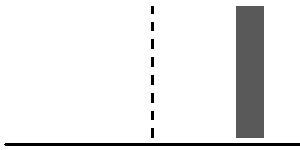
\includegraphics[width=0.06\textwidth]{../results/correlations/figures/posteriors/posterior_Real_lifted_case.pdf}     } 
		&   \multirow{2}{*}{  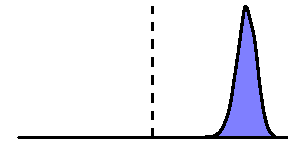
\includegraphics[width=0.06\textwidth]{../results/correlations/figures/posteriors/posterior_Efficiency_lifted_case.pdf}     } & \\
	&		\emph{to}            & \emph{a friend} &&&\\ \hline
	\multirow{2}{*}{\raisebox{.5pt}{\textcircled{\raisebox{-.9pt} {2}}}}	&copula    &    NP         
		&   \multirow{2}{*}{  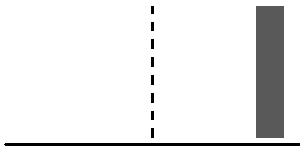
\includegraphics[width=0.06\textwidth]{../results/correlations/figures/posteriors/posterior_Real_lifted_cop.pdf}     } 
		&   \multirow{2}{*}{  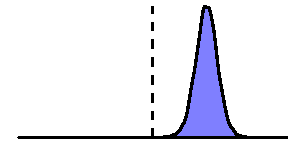
\includegraphics[width=0.06\textwidth]{../results/correlations/figures/posteriors/posterior_Efficiency_lifted_cop.pdf}     } & \\
	&	\emph{is}        & \emph{a friend}  &&&\\ \hline
	\multirow{2}{*}{\raisebox{.5pt}{\textcircled{\raisebox{-.9pt} {3}}}}	&auxiliary    &    VP       
		&   \multirow{2}{*}{  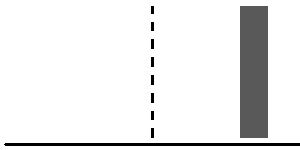
\includegraphics[width=0.06\textwidth]{../results/correlations/figures/posteriors/posterior_Real_aux.pdf}     } 
		&   \multirow{2}{*}{  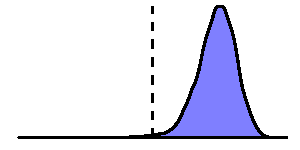
\includegraphics[width=0.06\textwidth]{../results/correlations/figures/posteriors/posterior_Efficiency_aux.pdf}     } & \\
	&	\emph{has}          & \emph{written}  &&&\\ \hline
	\multirow{2}{*}{\raisebox{.5pt}{\textcircled{\raisebox{-.9pt} {4}}}}	&noun    &    genitive      
		&   \multirow{2}{*}{  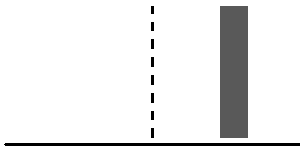
\includegraphics[width=0.06\textwidth]{../results/correlations/figures/posteriors/posterior_Real_nmod.pdf}     } 
		&   \multirow{2}{*}{  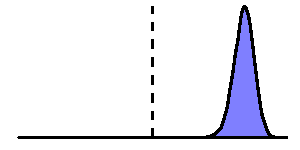
\includegraphics[width=0.06\textwidth]{../results/correlations/figures/posteriors/posterior_Efficiency_nmod.pdf}     } & \\
	&	\emph{friend} &  \emph{of John}  &&&\\ \hline
	\multirow{2}{*}{\raisebox{.5pt}{\textcircled{\raisebox{-.9pt} {5}}}}	&noun    &    relative clause      
		&   \multirow{2}{*}{  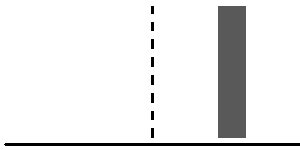
\includegraphics[width=0.06\textwidth]{../results/correlations/figures/posteriors/posterior_Real_acl.pdf}     } 
		&   \multirow{2}{*}{  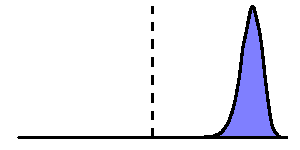
\includegraphics[width=0.06\textwidth]{../results/correlations/figures/posteriors/posterior_Efficiency_acl.pdf}     } & \\
	&	\emph{books} & \emph{that you read}  &&&\\ \hline
	\multirow{2}{*}{\raisebox{.5pt}{\textcircled{\raisebox{-.9pt} {6}}}}	&complementizer    &    S        
		&   \multirow{2}{*}{  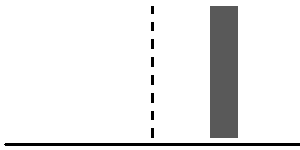
\includegraphics[width=0.06\textwidth]{../results/correlations/figures/posteriors/posterior_Real_lifted_mark.pdf}     } 
		&   \multirow{2}{*}{  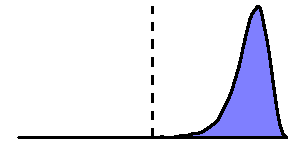
\includegraphics[width=0.06\textwidth]{../results/correlations/figures/posteriors/posterior_Efficiency_lifted_mark.pdf}     } & \\
	&	\emph{that} & \emph{she has arrived}  &&&\\ \hline
	\multirow{2}{*}{	\raisebox{.5pt}{\textcircled{\raisebox{-.9pt} {7}}}}	&verb    &    PP         
		&   \multirow{2}{*}{  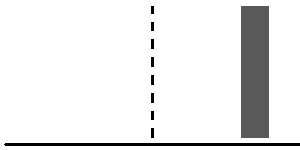
\includegraphics[width=0.06\textwidth]{../results/correlations/figures/posteriors/posterior_Real_obl.pdf}     } 
		&   \multirow{2}{*}{  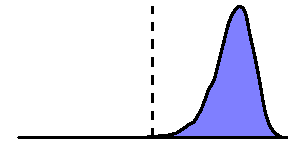
\includegraphics[width=0.06\textwidth]{../results/correlations/figures/posteriors/posterior_Efficiency_obl.pdf}     } & \\
	&	\emph{went} & \emph{to school}  &&&\\ \hline
	\multirow{2}{*}{\raisebox{.5pt}{\textcircled{\raisebox{-.9pt} {8}}}}	&want    &    VP        
		&   \multirow{2}{*}{  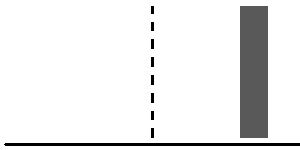
\includegraphics[width=0.06\textwidth]{../results/correlations/figures/posteriors/posterior_Real_xcomp.pdf}     } 
		&   \multirow{2}{*}{  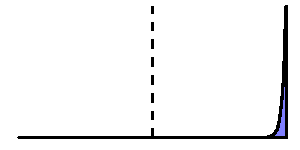
\includegraphics[width=0.06\textwidth]{../results/correlations/figures/posteriors/posterior_Efficiency_xcomp.pdf}     } & \\
	& \emph{wants}   &  \emph{to leave}  &&&\\ \hline
 \hline
\end{tabular}
	\end{center}
\caption{Efficiency optimization accurately predicts the Greenbergian correlations.
For each correlation, we provide the prevalence among the actual grammars of the 51 languages (left), and the posterior distribution of the prevalence among grammars optimized for efficiency (right).
Efficiency optimization predicts all eight correlations to hold in the majority of grammars.
}\label{table:corr-resu}
\end{table}









\begin{table}
	\begin{center}
\begin{tabular}{|c|cc||c|cc|ccccccc}
	\hline
	%&
	&        Real   &  Optimized &  & Real   &  Optimized  \\ \hline \hline 
	\multirow{2}{*}{\raisebox{.5pt}{\textcircled{\raisebox{-.9pt} {1}}}}	
				&   \multirow{2}{*}{  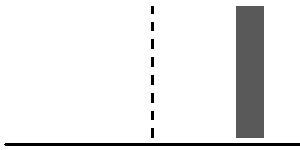
\includegraphics[width=0.06\textwidth]{../results/correlations/figures/posteriors/posterior_Real_lifted_case.pdf}     } 
		&   \multirow{2}{*}{  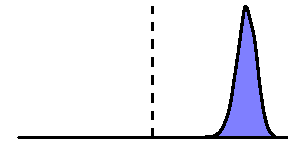
\includegraphics[width=0.06\textwidth]{../results/correlations/figures/posteriors/posterior_Efficiency_lifted_case.pdf}     } & \multirow{2}{*}{\raisebox{.5pt}{\textcircled{\raisebox{-.9pt} {5}}}}
		&   \multirow{2}{*}{  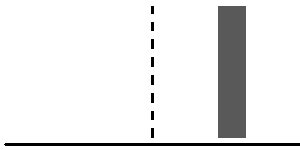
\includegraphics[width=0.06\textwidth]{../results/correlations/figures/posteriors/posterior_Real_acl.pdf}     } 
		&   \multirow{2}{*}{  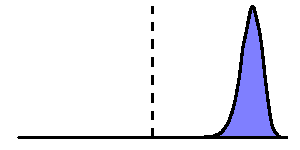
\includegraphics[width=0.06\textwidth]{../results/correlations/figures/posteriors/posterior_Efficiency_acl.pdf}     }  \\
	&	 &  &&&\\ \hline
	\multirow{2}{*}{\raisebox{.5pt}{\textcircled{\raisebox{-.9pt} {2}}}}
		&   \multirow{2}{*}{  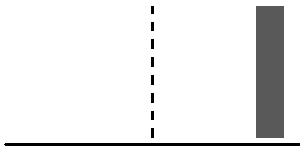
\includegraphics[width=0.06\textwidth]{../results/correlations/figures/posteriors/posterior_Real_lifted_cop.pdf}     } 
		&   \multirow{2}{*}{  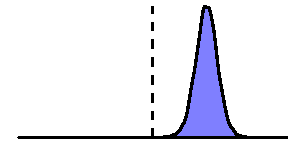
\includegraphics[width=0.06\textwidth]{../results/correlations/figures/posteriors/posterior_Efficiency_lifted_cop.pdf}     } & 	\multirow{2}{*}{\raisebox{.5pt}{\textcircled{\raisebox{-.9pt} {6}}}}
		&   \multirow{2}{*}{  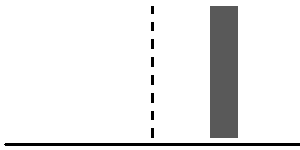
\includegraphics[width=0.06\textwidth]{../results/correlations/figures/posteriors/posterior_Real_lifted_mark.pdf}     } 
		&   \multirow{2}{*}{  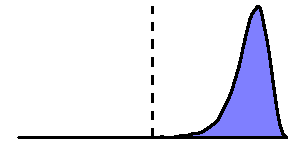
\includegraphics[width=0.06\textwidth]{../results/correlations/figures/posteriors/posterior_Efficiency_lifted_mark.pdf}     }\\
	&	 &  &&&\\ \hline
	\multirow{2}{*}{\raisebox{.5pt}{\textcircled{\raisebox{-.9pt} {3}}}}
		&   \multirow{2}{*}{  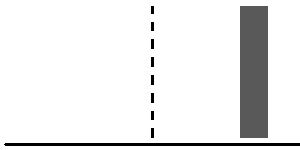
\includegraphics[width=0.06\textwidth]{../results/correlations/figures/posteriors/posterior_Real_aux.pdf}     } 
		&   \multirow{2}{*}{  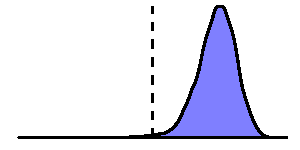
\includegraphics[width=0.06\textwidth]{../results/correlations/figures/posteriors/posterior_Efficiency_aux.pdf}     } & \multirow{2}{*}{	\raisebox{.5pt}{\textcircled{\raisebox{-.9pt} {7}}}}
		&   \multirow{2}{*}{  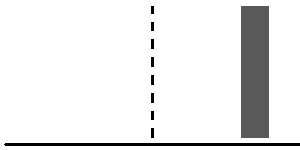
\includegraphics[width=0.06\textwidth]{../results/correlations/figures/posteriors/posterior_Real_obl.pdf}     } 
		&   \multirow{2}{*}{  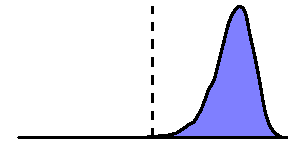
\includegraphics[width=0.06\textwidth]{../results/correlations/figures/posteriors/posterior_Efficiency_obl.pdf}     }\\
	&	 &  &&&\\ \hline
	\multirow{2}{*}{\raisebox{.5pt}{\textcircled{\raisebox{-.9pt} {4}}}}
		&   \multirow{2}{*}{  \includegraphics[width=0.06\textwidth]{../results/correlations/figures/posteriors/posterior_Real_nmod.pdf}     } 
		&   \multirow{2}{*}{  \includegraphics[width=0.06\textwidth]{../results/correlations/figures/posteriors/posterior_Efficiency_nmod.pdf}     } & \multirow{2}{*}{\raisebox{.5pt}{\textcircled{\raisebox{-.9pt} {8}}}}	
		&   \multirow{2}{*}{  \includegraphics[width=0.06\textwidth]{../results/correlations/figures/posteriors/posterior_Real_xcomp.pdf}     } 
		&   \multirow{2}{*}{  \includegraphics[width=0.06\textwidth]{../results/correlations/figures/posteriors/posterior_Efficiency_xcomp.pdf}     }\\
	&	 &  &&&\\ \hline
 \hline
\end{tabular}
	\end{center}
\caption{\textcolor{red}{choose this or the other version}Efficiency optimization accurately predicts the Greenbergian correlations.
For each of the eight correlations (Table~\ref{table:corr-dryer}), we provide the prevalence among the actual grammars of the 51 languages (left), and the posterior distribution of the prevalence among grammars optimized for efficiency (right).
Efficiency optimization predicts all eight correlations to hold in the majority of grammars.
}\label{table:corr-resu}
\end{table}


